\documentclass[a4paper]{article}
\usepackage[T1]{fontenc}
\usepackage[utf8]{inputenc}
\usepackage[italian]{babel}
\usepackage{geometry}
\geometry{a4paper,top=1cm,bottom=2cm,left=1.5cm,right=1cm,bindingoffset=5mm}

\usepackage[italian]{varioref} %per ottenere il package varioref in lingua italiana
% \usepackage{hyperref} % per i collegamenti esterni alla pagina
\usepackage[colorlinks]{hyperref} % per ottenere i collegamente interni ed esterni alla pagina colorati
% \hypersetup{hidelinks} % per nascondere i collegamenti

%
% CREARE UN COMANDO PER MANDARE LE EMAIL
%
\newcommand{\mail}[1]{\href{mailto:#1}{\texttt{#1}}}
%
% è stato appena creato il comando \mail


\usepackage{graphicx} % per utilizzare le immagini


\title{doc10}
\author{Antonio Maulucci}
\date{February 2017}

\begin{document}

\maketitle

\section{I Link interni}
\label{sec:rif-one} %label di riferimento

Questa è la prima sezione del documento

\subsection{sub1}
\subsection{sub2}
\subsection{sub3}

\newpage

\section{Richiamo dei link interni}

In questa sezione vediamo come creare un link interno verso il paragrafo~\ref{sec:rif-one}

Abbiamo chiamato il paragrafo \vref{sec:rif-one} % funzione del package varioref che stampa il numero del dato a cui si riferisce e la sua pagina di appartenenza nella lingua specificata quando si dichiarato il package


\section{Collegamenti al Web}

Questo è un \href{http://www.antomau.com}{riferimento al mio sito web personale}

\subsection{I collegamenti ad un sito}

Per scrivere esplicitamente un collegamento usare la funzione url importata dal package hyperref: \url{http://www.antomau.com}

\section{Invio di un eMail ad un indirizzo di posta}
% usare il comando \mail creato in precedenza
Contattami a: \mail{prova.prova@prova.com}





\newpage

\section{Stile e corpo del testo}

\subsection{Modificare lo stile}

La seguente parola è scritta in \textit{corsivo} ma il resto del testo no! %corsivo
\\\\
La seguente parole è scritta in \textbf{grassetto} ma il resto del testo no! %grassetto
\\\\
La seguente parola è scritta in \textit{\textbf{grassetto-corsivo}} ma il resto del testo no! %grassetto-corsivo
\\\\
testo in stile \texttt{macchina da scrivere}
\\\\
testo \em{evidenziato}
\\\\
testo in \scshape{maiuscoletto}
\\\\
testo \slshape{inclinato}
\\\\
testo \rmfamily{tondo}
\\\\
testo \sffamily{senza grazie}

Altri testi alla pagina 48 del manuale Arte \LaTeX\ .

\subsection{Modificare il corpo}

È già stato visto come modificare il corpo del testo nella sezione \textit{Headers}.

\vspace{3cm}

\section{Le immagini e la grafica}

\subsection{Formati supportati}

Tutte le immagini inserite vengono convertite in immagini vettoriali.
\\\\
Formati supportati:
\\\\
\begin{tabular}{|c|}
\hline
pdf\\
\hline\\
jpeg\\
\hline\\
png\\
\hline\\
eps\\
\hline
\end{tabular}

\subsection{Inserire un immagine}

Per inserire un immagine si usa il comando:

\begin{verbatim}
    \includegraphics[<chiave>=<valore>]{<immagine>}
\end{verbatim}

dove la chiave è uno specifico elemento

e il valore il valore della chiave.

\begin{tabular}{r|l}
\hline\\
chiave & elemento su cui agisce\\
\hline\\
width & largezza dell'immagine\\
height & altezza dell'immagine (non si può usare insieme a width)\\
scale & Larghezza e altezza\\
angle & orientamento dell'immagine
\end{tabular}




\newpage


\subsection{Includere un immagine}

Il nome dell'immagine (secondo parametro di includegrapghic) non deve contenere l'estensione del file

\begin{center}
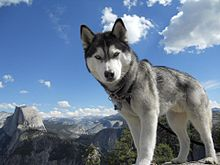
\includegraphics[width=7cm]{siberian}
\end{center}

Didascalie e disposizioni a pagina 106 del manuale Arte \LaTeX\ .


\vspace{4cm}
\begin{center}
\copyright \sffamily{Antonio Maulucci 2017}
\end{center}
\end{document}
